
\documentclass{article}
\usepackage{fullpage}
\usepackage{color}
\usepackage[normalem]{ulem}
\usepackage{hyperref}
\usepackage{enumitem}
\usepackage{graphicx}
\hypersetup{colorlinks}
\hyphenpenalty=100000
\begin{document}
\setlength{\voffset}{3.5in}
\title{Project Documentation}
\author{\Large Android Based Situational Awareness: Moving Map\\
Tom Atnip, Susi Cisneros, Sam Kim, and Seth Troisi}
\date{\today}
\maketitle
\clearpage
\setlength{\voffset}{0pt}
\tableofcontents
\clearpage
~\\
\begin{Large}\textbf{Changes}\end{Large}\\
~\\
\begin{tabular}{ | p{1.5in} | p{4.5in} | }
\hline
\textbf{Date} & \textbf{Description}\\
\hline
\hline
September 13, 2012 & Document started\\
\hline
September 13, 2012 & Wrote Requirements and Questions to ask Raytheon\\
\hline
September 20, 2012 & Created outline\\
\hline
September 20, 2012 & Wrote Users/Stakeholders section\\
\hline
September 23, 2012 & Wrote Key Needs, Alternatives, Risks, Documentation Metrics, and Code Metrics\\
\hline
September 24, 2012 & Updated Requirements as per Gate 5 visit with Raytheon\\
\hline
October 8, 2012 & Revised Requirements, added Assumptions and Opportunities, and updated Risks\\
\hline
October 15, 2012 & Added Introduction and made Requirements into shall statements\\
\hline
October 25, 2012 & Updated Requirement, added Performance Requirements\\
\hline
November 7, 2012 & Updated Performance placeholder\\
\hline
January 26, 2013 & Project Document Audit\\
\hline
\end{tabular}
\clearpage

\section{Introduction}
This document details all documentation associated with this project.  It includes the problem statement, requirements, project plan, and metrics.

\section{Problem Statement}
\subsection{User/Stakeholder Descriptions}
\subsubsection{Users} 
\textbf{Soldier, Police Officers, and other Ground Personnel}\\
The users of our program are seeking to maintain their situational awareness in locations which may not have connectivity to the Internet.  Many of them use voice guided situational awareness technology, but in light of advances in mobile devices, they could receive this information in a visual manner.  

\subsubsection{Stakeholders}
\textbf{Raytheon}\\
Raytheon's customers are mainly military organizations, many of which are using Raytheon's current situational awareness technologies.  Raytheon is looking to update these technologies to keep their position as a leading provider of military systems.\\ \\
\textbf{JD Hill}\\
JD is the client who proposed this solution.  He is a major proponent of using mobile devices in a military application.\\ \\
\textbf{Doug Dusseau}\\
Doug is the acting Technical Lead for this project. \\ \\
\textbf{Development Team}\\
The development team on this project are graduating seniors who wish to learn more about the software development process and interaction with a client.  They are very interested in learning more about developing on the Android platform.

\subsection{Key Needs}

\begin{tabular}{ | p{.5in} | p{4.5in} | }
\hline
\textbf{ID} & \textbf{Need}\\
\hline
\hline
N0 & View map of surrounding area\\
\hline
N1 & View points of interest on the map\\
\hline
N2 & View current location on the map\\
\hline
N3 & Map must not require internet access\\
\hline
N4 & Map must be Android based\\
\hline
N5 & Application must work on any size android device\\
\hline
\end{tabular}


\subsection{Current Solution}

\subsection{Alternatives}
All considered solutions to the proposed system require Internet access.

\section{Requirements}

\subsection{Functional}

\begin{tabular}{ | p{.5in} | p{4.5in} | p{1in}|}
\hline
\textbf{ID} & \textbf{Requirement} & \textbf{Priority}\\
\hline
\hline
FR0 & The system shall let the user pan the map by a dragging gesture & Objective\\
\hline
FR1 & The system shall let the user zoom using an on-screen button & Threshold\\
\hline
FR2 & The system shall let the user zoom using pinch gestures & Objective\\
\hline
FR3 & The system shall let the user zoom using double tap & Objective\\
\hline
FR4 & The system shall store map tiles on the device & Threshold\\
\hline
FR5 & The system shall display map tiles which are stored on the device & Threshold\\
\hline
FR6 & The system shall be able to pull map tiles which are stored on a local server and store them on the device & Objective\\
\hline
FR7 & The system shall georeference the location of the device & Threshold\\
\hline
FR8 & The system shall let the user center on current location & Objective\\
\hline
FR9 & The system shall store multiple map types & Threshold\\
\hline
FR10 & The system shall let the user choose the map type & Objective\\
\hline
FR11 & The system shall store points of interest as a map overlay & Objective\\
\hline
FR12 & The system shall display points of interest overlays & Objective\\
\hline
FR13 & The system shall let the user choose which overlays are displayed & Objective\\
\hline
FR14 & The system shall let the user add custom points of interest & Objective\\
\hline
FR15 & The system shall let the user choose which overlay the custom point of interest is added to & Objective\\
\hline
FR16 & The system shall let the user create new overlays & Objective\\
\hline
FR17 & The system shall display a compass & Threshold\\
\hline
FR18 & The system shall let the user toggle heading/north up & Threshold\\
\hline
FR19 & The system shall let the user change default settings via a settings menu found in the menu bar & Threshold\\
\hline
FR20 & The system shall let the user access a help menu via the menu bar & Objective\\
\hline
\end{tabular}

\subsection{Non-functional}

\begin{tabular}{ | p{.5in} | p{5in} | }
\hline
\textbf{ID} & \textbf{Requirement}\\
\hline
\hline
NR0 & The system shall run on Android platforms running at least version 3.0 (Honeycomb)\\
\hline
NR1 & The system shall receive GPS data from a local server or the device\\
\hline
NR2 & The system shall display properly on either mobile phones or tablets\\
\hline
NR3 & The system shall use modular code\\
\hline
NR3 & The system shall use the Android usability conventions\\
\hline
\end{tabular}

\subsection{Performance}

\begin{tabular}{ | p{.5in} | p{5in} | }
\hline
\textbf{ID} & \textbf{Requirement}\\
\hline
\hline
PR0 & To be determined\\
\hline
\end{tabular}


\section{Project Plan}
\subsection{Schedule}
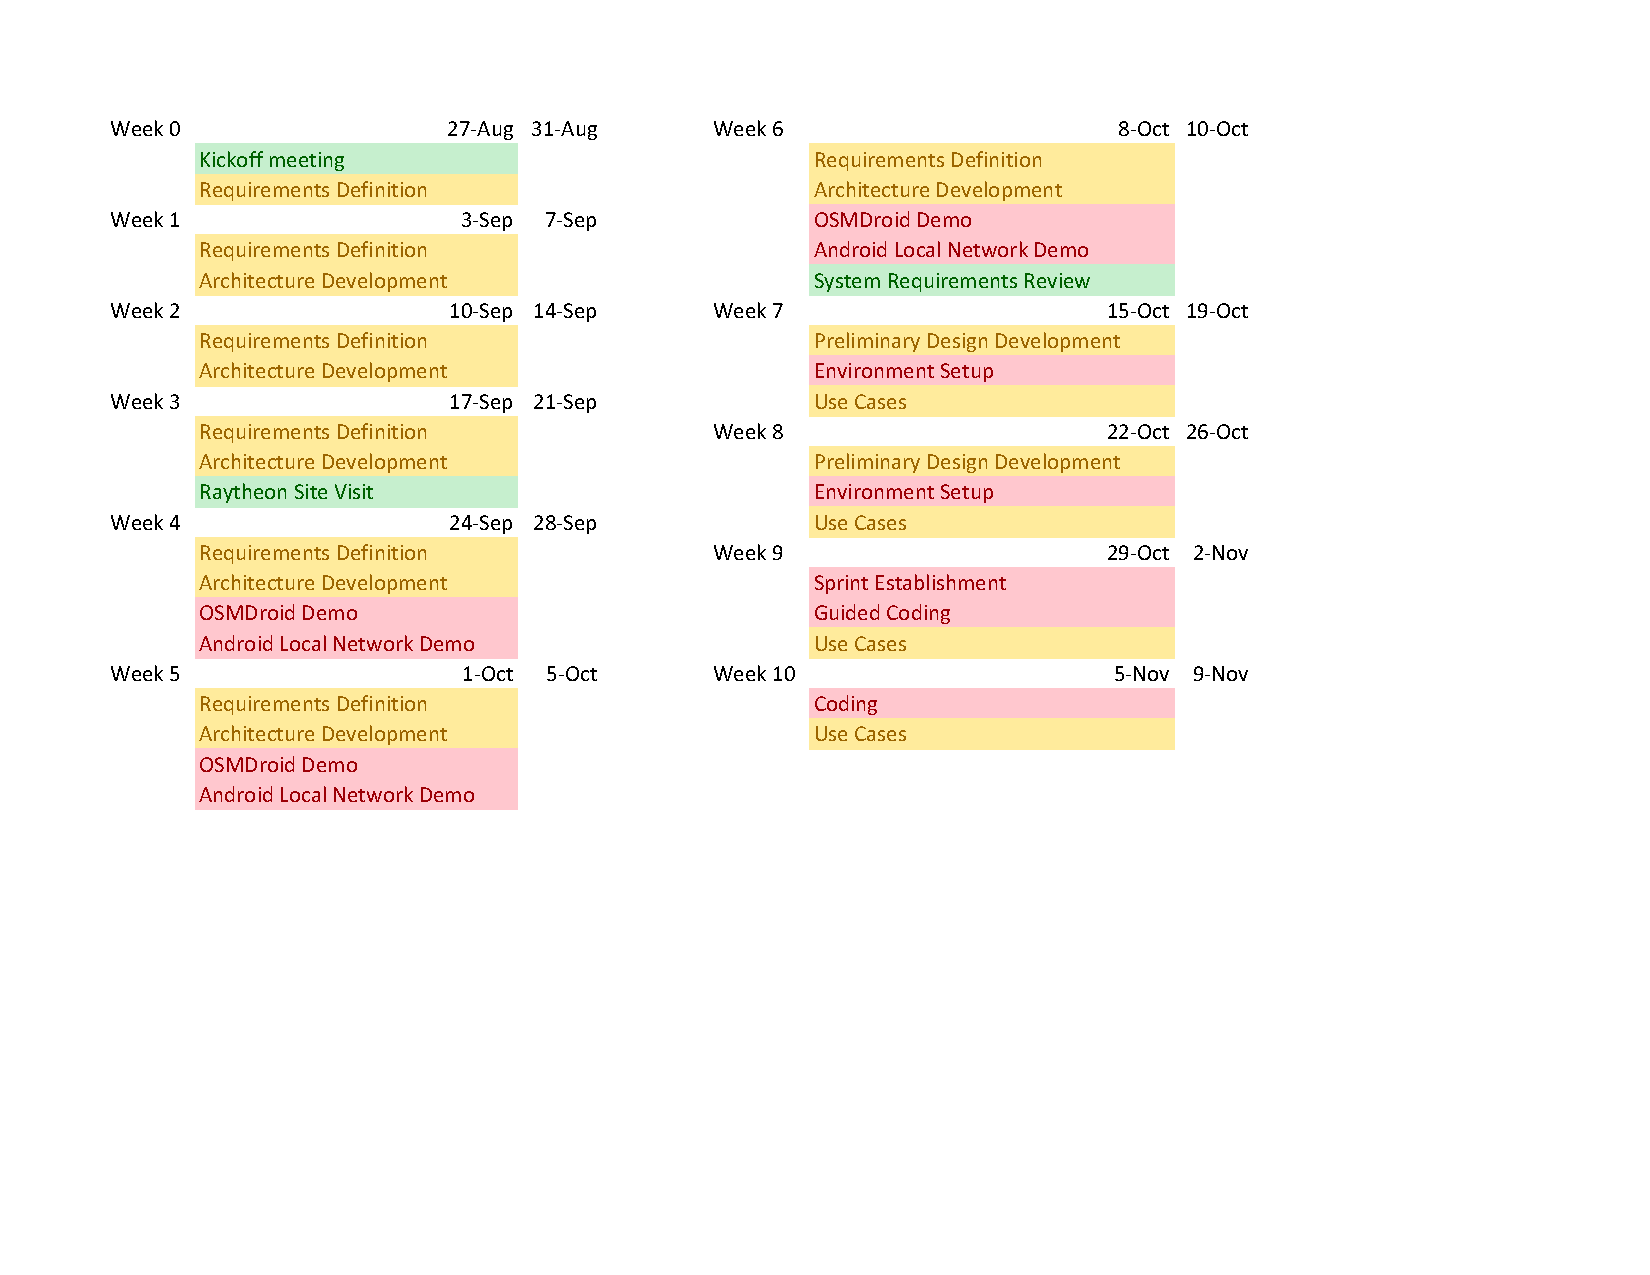
\includegraphics[keepaspectratio, width=8in]{Schedule/FallSchedule.pdf} \\

\subsection{Assumptions}
\begin{tabular}{ | p{.5in} | p{4.5in} | }
\hline
\textbf{ID} & \textbf{Assumption}\\
\hline
\hline
A0 & There exists an open source mapping engine for Android devices\\
\hline
A1 & The mapping engine does not require an internet connection to run\\
\hline
A2 & Android devices can connect to a local server\\
\hline
\end{tabular}

\subsection{Risks}
\begin{tabular}{ | p{.5in} | p{4.5in} | }
\hline
\textbf{ID} & \textbf{Risk}\\
\hline
\hline
R0 & Performance of the system\\
\hline
R1 & Organizing data in the correct format in a timely manner\\
\hline
\end{tabular}

\subsection{Opportunities}
\begin{tabular}{ | p{.5in} | p{4.5in} | }
\hline
\textbf{ID} & \textbf{Opportunity}\\
\hline
\hline
O0 & Finding a feature complete mapping engine\\
\hline
\end{tabular}

\section{Metrics}
\subsection{Project}
\subsubsection{Documentation}
The progress of the documentation will be tracked by breaking it down into three parts: the percent written and ready for review, the percent that has been reviewed, and the percent that is ready for delivery. The initial portion will encompass the percentage of the requirements, features, and other material that have been documented according to our currently known goals. A portion of the documentation will be considered in the reviewed stage once Dr. Wollowski and/or JD Hill have provided feedback and approval. Once a section of the documentation is in its final state (written, reviewed, and stable), it will be considered complete.\\ \\
\begin{tabular}{l r}
Percent Written: & 100 \\
Percent Reviewed: & 100 \\
Percent Complete: & 100 \\
\end{tabular}
\subsubsection{Code}
During the coding phase of this project, progress will be tracked by the features scheduled during an iteration and the number of features completed. Code will belong to one of five phases – unwritten, written, peer reviewed, tested, or complete. Once code has been written and passes the required unit tests, it will undergo a peer review to check for good coding practices, clarity, and errors. After a peer review the functionality will then be required to pass integration tests. Once it has passed system integration, it will be considered complete and will be merged into the main branch of code.\\ \\
\begin{tabular}{l r}
Percent Written: & 30 \\
Percent Reviewed: & 15 \\
Percent Tested: & 0 \\
Percent Complete: & 0 \\
\end{tabular}
\subsubsection{Testing}
For the final phase of the project, progress will be measured by how many tests are passing. The tests that the software will be subjected to will be more thorough than the tests required for code to join the main branch. Most tests will be automated, but there will also be human factor tests.\\ \\
\begin{tabular}{l r}
Percent Passing: & 0 \\
\end{tabular}
\subsection{Process}
The process that the project is following will be measured by due dates met versus missed due dates.\\ \\
\begin{tabular}{l r}
Milestone Dates Kept: & 0 \\
\end{tabular}

\subsection{Communication}
Communication will be measured by how well the team feels that their needs are being heard and being taken care of, along with efficiency of meetings.\\ \\
\begin{tabular}{l r}
Team Confidence: & 85 \\
Meetings: & 95 \\
\end{tabular}

\clearpage

\section{Questions}

\begin{enumerate}[label*=6.\arabic*]
\item
\end{enumerate}


\end{document}